\newpage
\section{引论}
\subsection{什么是编译原理}

计算机上执行一个高级语言程序通常分为两步:第一步,用一个编译程序把高级语言翻译成机器语言程序;第二部,运行所得到的机器语言程序求计算结果。

通常所说的翻译程序是这样一个程序,它能够把某一种语言程序(称为源语言程序)转换成另一种语言程序(称为目标语言程序),前后者逻辑上是等价的。这样的一个翻译程序就称为编译程序。

高级语言除了先编译后执行外,有时也可``解释''执行。一个源语言的解释程序就是这样的程序,它以该语言写的源程序作为输入,但不产生目标程序,而是边解释边执行源程序本身。

\subsection{编译过程概述}

编译程序的工作过程一般可分为五个阶段:词法分析,语法分析,语义分析与中间代码产生,优化,目标代码生成。

\noindent\textbf{词法分析}

词法分析的任务是:输入源程序,对构成源程序的字符串进行扫描和分解,识别出一个个单词。这一过程类似于英文翻译中认识每一个单词的意义。

\noindent\textbf{语法分析}

语法分析的任务是:在词法分析的基础上,根据语言的语法规则,把单词符号串分解成各类语法单位,如``短语'',``子句'',``句子'',``程序段''等。通过语法分析,确定整个输入串是否构成语法上正确的``程序''。语法分析所依循的是语言的语法规则。语法规则通常用上下文无关文法描述。词法分析是一种线性分析,而语法分析是一种层次结构分析。

\noindent\textbf{语义分析和中间代码产生} (例子见书 P3)

这一阶段的任务是:对语法分析所识别出的各类语法范畴,分析其含义,并进行初步翻译(产生中间代码)。这一阶段通常包括两个方面的工作。首先,对每种语法范畴进行静态语义检查。如果语义正确,则进行另一方面工作,即进行中间代码的翻译。这一阶段所依循的是语言的语义规则。通常使用属性文法描述语义规则。

``翻译''仅仅在这里才开始涉及到。所谓的``中间代码''是一种含义明确,便于处理的记号系统,它通常独立于具体的硬件。

\noindent\textbf{优化}

优化的的任务在于对前端产生的中间代码进行加工变换,以期在最后阶段能产生更为高效(省时间省空间)的目标代码。优化的主要方面有:公共子表达式的提取,循环优化,删除无用代码等等。有时为了便于``并行运算'',还可对代码进行并行化处理。优化所依循的原则是程序的等价变换规则。

\noindent\textbf{目标代码生成}

这一阶段的任务是:把中间代码(优化处理过后)变换成特定机器上的低级语言代码。这阶段实现了最后的翻译,它的工作有赖于硬件系统结构和机器指令含义。

目标代码的形式可以是绝对指令代码或可重定位的指令代码或汇编指令代码。如目标代码是绝对指令代码,则这种目标代码可立即执行。如目标代码是汇编指令代码,则需汇编器汇编后才能进行。

现代多数编译程序产生的是可重定位的指令代码。这种目标代码在运行前必须借助一个连接装配程序把各个目标模块(包括系统提供的库模块)连接在一起。确定程序变量(常数)在主存中的位置,装入内存中指定的起始地址,使之称为一个可运行的绝对指令代码程序。

\subsection{编译程序的结构}
\subsubsection{编译程序总框}

\begin{figure}[H]
    \centering
    \begin{tikzpicture}[scale=1,thick,node font=\small]
        \node at (-5,4) [draw, text width=12pt, minimum width=1cm , minimum height = 9cm] {表格管理};
        \node at (5,4) [draw, text width=12pt, minimum width=1cm , minimum height = 9cm] {出错处理};

        \begin{scope}[every node/.style = {draw,minimum width = 6cm, minimum height = 1cm}]
            \node at (0,8) {词法分析器(扫描器)};
            \node at (0,6) {语法分析器(分析器)};
            \node at (0,4) {语义分析与中间代码产生器};
            \node at (0,2) {优化器};
            \node at (0,0) {目标代码生成器};
        \end{scope}

        \foreach \x in {8,6,4,2,0}
            \draw [<->,>=Stealth] (-4.5,\x) -- (-3,\x);
        \foreach \x in {8,6,4,2,0}
            \draw [<->,>=Stealth] (4.5,\x) -- (3,\x);

        \begin{scope}[every node/.style = {right = 0.5cm,pos=0.5}]
            \draw [->,>=Stealth] (0,9.5) -- (0,8.5) node {源程序};
            \draw [->,>=Stealth] (0,7.5) -- (0,6.5) node {单词符号};
            \draw [->,>=Stealth] (0,5.5) -- (0,4.5) node {语法单位};
            \draw [->,>=Stealth] (0,3.5) -- (0,2.5) node {中间代码};
            \draw [->,>=Stealth] (0,1.5) -- (0,0.5) node {中间代码};
            \draw [->,>=Stealth] (0,-0.5) -- (0,-1.5) node {目标代码};
        \end{scope}

    \end{tikzpicture}
    \caption{编译程序总框}
    \label{编译程序总框}
\end{figure}

有的编译程序在识别出各类语法单位后,构造并输出一棵表示语法结构的语法树,然后,根据语法树进行语义分析和中间代码产生。还有许多编译程序在识别出语法单位后并不真正构造语法树,而是调用相应的语义子程序。在这种编译程序中,扫描器,分析器和中间代码产生器并非截然分开,而是相互穿插。

\subsubsection{表格与表格管理}

编译程序在工作过程中需要保持一系列的表格,以登记源程序的各类信息和编译各阶段的进展情况。在编译程序使用的各种表格中,最重要的是符号表。它用来登记源程序中出现的每个名字以及名字的各种属性。

编译各阶段都涉及到构造,查找或更新有关表格。

\subsubsection{出错处理}

编译程序应能对出现在源程序中的错误进行处理。这部分工作由专门的一组程序(出错处理程序)完成。一个好的编译程序应找到错误,并最小化错限制错误造成的影响,使得源程序的其他部分能够继续被编译,以便进一步发现其他可能的错误。

编译过程的每一阶段都可能检测出错误,绝大部分错误出现在编译的前三阶段。源程序中的错误通常可分为语法错误与语义错误两大类。

\begin{itemize}
    \item 语法错误 
    
    指源程序中不符合语法(词法)规则的错误,可在语法分析与词法分析时检测出来。例如非法字符,括号不匹配等。
    \item 语义错误
    
    指源程序中不符合语义规则的错误,一般在语义分析时检测出来,有的语义错误需要在运行时检测出来。例如类型不一致,作用域错误等
\end{itemize}

\subsubsection{遍}

编译过程具体实现时,受不同限制,往往将编译程序组织为若干遍(pass)。所谓``遍''就是对源程序或源程序中间结果从头到尾扫描一次,并作有关的加工处理,生成新的中间结果或目标程序。通常,每遍地工作由从外存上获得地前一遍地中间结果开始,完成它所含地有关工作之后,再把结果记录于外存。既可以将几个不同阶段合为一遍,也可以把一个阶段的工作分为若干遍。

遍数多一点有一个好处,即整个编译程序的逻辑结构可能清晰一点。但遍数多势必增加输入/输出所消耗的时间。

\subsubsection{编译前端与后端}

概念上,我们有时把编译程序分为编译前端和编译后端。前端主要由与源语言有关但与目标无关的部分组成。包括:词法分析,语法分析,语义分析与中间代码产生,有的代码优化工作也能包含在内。后端包括编译程序中与目标机有关的那部分,如与目标机有关的代码优化和目标代码生成等。通常,后端不依赖于源语言而仅依赖于中间语言。

可以取编译程序的前端,改写其后端以生成不同目标机上的相同语言的编译程序。也可以将几种源语言编译成相同的中间语言,然后为不同的前端配上相同的后端。

\subsection{编译程序与程序设计环境}

程序设计环境:编译程序与程序设计工具一起构成。程序设计工具包括:编辑程序,连接程序,调试工具等。

集成化的程序设计环境:特点是将相互独立的程序设计工具集成起来,以便为程序员提供完整的,一体化的支持,从而进一步提高程序开发效率,改善程质量。

下面以 Ada 语言的程序设计环境 APSE 为例,介绍程序设计环境的基本构成与主要工具。

\begin{figure}[H]
    \centering
    \begin{tikzpicture}[scale = 1,thick,every node/.style = {node font = \small}]
        \draw (0,0) circle [radius=4.7cm] circle [radius = 2cm] circle [radius = 1cm];
        \draw [rotate = -60] (3.7cm,0) arc [start angle = 0,end angle = 315,radius=3.7cm];

        \begin{scope}
            \node at (0,0) {宿主机};
            \node at (0,1.5) {KAPSE};
            \node at (0,4.2) {APSE};
        \end{scope}

        \foreach \angle in {-60,-15,30,75,120,165,210,255}
            \draw (\angle:2) -- (\angle:3.7);

        \begin{scope} [every node/.style = {text width = 24.5pt}]
            \node at (-35:2.7) {连接程序};
            \node at (10:2.7) {调试程序};
            \node at (55:2.7) {编译程序};
            \node at (100:2.7) {MAPSE\\$\cdots$};
            \node at (145:2.7) {编辑程序};
            \node [text width = 42pt] at (190:2.7) {配置管理程序};
            \node [text width = 42pt] at (235:2.7) {命令解释程序};
        \end{scope}

        \begin{scope} [gray,every node/.style = {black,draw,circle,fill=white}]
            \draw [<-,>=Stealth] (35:2cm) -- (35:8cm) node {工具界面};
            \draw [<-,>=Stealth] (-25:4.7cm) -- (-25:8cm) node {用户界面};
        \end{scope}
    \end{tikzpicture}
    \caption{Ada 程序设计环境}
    \label{Ada 程序设计环境}
\end{figure}

最内层是宿主计算机系统,包括硬件,宿主操作系统和其他支撑软件;
第一层是核心 APSE (KAPSE),包含环境数据库,通信即运行时支撑功能等。
第二层,最小 APSE (MAPSE),包含 Ada 程序开发及维护的基本工具,这些工具包括编译程序,编辑程序,连接程序,调试程序等。
第三层,APSE,在 MAPSE 外面再机上更广泛的工具构成完整的 APSE。

在一个程序设计环境中,编译程序起着中心作用。连接程序,调试程序等的工作直接依赖于编译程序所产生的结果。而其他工具的构造常常要用到编译的原理,方法和技术。

\subsection{编译程序的生成}

我们用一种 T 形图来表示源语言 S,目标语言 T 和编译程序实现语言 I 之间的关系。

\begin{figure}[H]
    \centering
    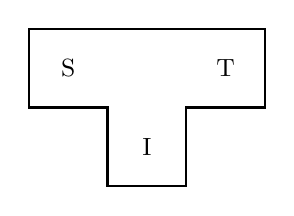
\begin{tikzpicture}[scale = 1,thick,every node/.style = {node font = \small}]
        \draw (0,1) -- (1,1) -- (1,0) --(2,0) -- (2,1) -- (3,1) -- (3,2) -- (0,2) -- cycle;
        \node at (1.5,0.5) {I};
        \node at (0.5,1.5) {S};
        \node at (2.5,1.5) {T};
    \end{tikzpicture}
    \caption{T形图}
    \label{T形图}
\end{figure}

如果 A 机器上已有一个用 A 机器代码实现的某高级语言 $L_1$ 的编译程序,则我们可以用 $L_1$ 语言编写另一种高级 $L_2$ 的编译程序,把学好的 $L_2$ 编译程序经过 $L_1$ 编译程序编译后就可得到 A 机器代码实现的 $L_2$ 编译程序。

\begin{figure}[H]
    \centering
    \begin{tikzpicture}[scale = 1,thick,every node/.style = {font = {\scriptsize \bfseries}}]
        \foreach \x/\y in {0/0,-2/1,2/1}
            \draw (\x,\y+1) -- (\x+1,\y+1) -- (\x+1,\y) --(\x+2,\y) -- (\x+2,\y+1) -- (\x+3,\y+1) -- (\x+3,\y+2) -- (\x,\y+2) -- cycle;
        \node at (1.5,0.5) {A代码};
        \node at (0.6,1.5) {$L_1$语言};
        \node at (2.4,1.5) {A代码};

        \node at (-0.5,1.5) {$L_1$语言};
        \node at (-1.4,2.5) {$L_2$语言};
        \node at (0.4,2.5) {A代码};

        \node at (3.5,1.5) {A代码};
        \node at (2.6,2.5) {$L_2$语言};
        \node at (4.4,2.5) {A代码};
    \end{tikzpicture}
    \caption{用 $L_1$ 语言编写编译程序}
    \label{用 $L_1$ 语言编写编译程序}
\end{figure}

采用一种所谓 ``移植'' 方法,我们可以利用 A 机器上已有的高级语言 L 编写一个能够在 B 机器上运行的高级语言 L 的编译语言,然后把该源程序经过 A 机器上的 L 编译程序编译后得到能在 A 机器上运行的产生 B 机器代码的编译程序,用这个编译程序再一次编译上述编译程序源程序就得到了能在 B 机器上运行的产生 B 机器代码的编译程序。

\begin{figure}[H]
    \centering
    \begin{tikzpicture}[scale = 1,thick,every node/.style = {font = {\scriptsize \bfseries}}]
        \foreach \x/\y in {0/0,-2/1,2/1,0/2,4/2}
            \draw (\x,\y+1) -- (\x+1,\y+1) -- (\x+1,\y) --(\x+2,\y) -- (\x+2,\y+1) -- (\x+3,\y+1) -- (\x+3,\y+2) -- (\x,\y+2) -- cycle;
        \node at (1.5,0.5) {A代码};
        \node at (0.6,1.5) {L语言};
        \node at (2.4,1.5) {A代码};

        \node at (-0.5,1.5) {L语言};
        \node at (-1.4,2.5) {L语言};
        \node at (0.4,2.5) {A代码};

        \node at (3.5,1.5) {A代码};
        \node at (2.6,2.5) {L语言};
        \node at (4.4,2.5) {A代码};

        \node at (1.5,2.5) {L语言};
        \node at (0.6,3.5) {L语言};
        \node at (2.4,3.5) {B代码};

        \node at (5.5,2.5) {B代码};
        \node at (4.6,3.5) {L语言};
        \node at (6.4,3.5) {B代码};
    \end{tikzpicture}
    \caption{编译程序``移植''}
    \label{编译程序``移植''}
\end{figure}

自编译方法:先对语言的核心部分构造一个小小的编译程序(可用低级语言实现),再以它为工具构造一个能够编译更多语言成分的较大编译程序。如此扩展下去,就能像滚雪球一样,越滚越大。通过这一系列自展途径而形成编译程序的过程叫做自编译过程。

在某一台机器上为某种语言构造一个编译程序,必须掌握以下内容:
\begin{enumerate}
    \item 源语言:对被编译的源语言,要深刻理解其结构(语法)和含义(语义)。
    \item 目标语言:假定目标语言是机器语言,那么就必须搞清楚硬件的系统结构和操作系统的功能。
    \item 编译方法:把一种语言程序翻译为另一种语言程序方法很多,但必须准确地掌握一二。
\end{enumerate}